\chapter{Results}
\label{cha:fifth_chapter}
In this chapter we will first introduce the methodology we used to evaluate our models and then we will show and discuss the results we have obtained both in classifying the diseases and in localizing them. 

\section{Evaluation Criteria}
\label{sec:evaluation_criteria}
As introduced in Chapter \ref{cha:third_chapter}, the dataset already provides a subset of 202 frontal images that can be used to asses the performances of the models. We decided, in our work, to evaluate our models using the same subset, in order to be able to compare our results with that carried out by related works.
The performance, however, have not been evaluated over the entire set of pathologies but, instead, only 5 of them (\textit{Atelectasis}, \textit{Cardiomegaly}, \textit{Consolidation}, \textit{Edema}, \textit{Pleural Effusion}) have been taken into consideration, based on their clinical significance and presence in the dataset. 

\subsubsection{AUROC}
\ac{AUROC} is the summary metric we used to assess the goodness of our classifiers. In order to define it, we have to first introduce some quantities that are largely used to measure the performance of a classifier:
\begin{itemize}
    \item \ac{TP}: outcome \textit{correctly} classified as \textit{positive}
    \item \ac{TN}: outcome \textit{correctly} classified as \textit{negative}
    \item \ac{FP}: outcome \textit{incorrectly} classified as \textit{positive}
    \item \ac{FN}: outcome \textit{incorrectly} classified as \textit{negative}
\end{itemize}

We can now introduce the notion of Receiving Operating Characteristic, that is a curve plotting the \ac{TPR} against the \ac{FPR}. \ac{TPR}, also known as sensitivity or recall, measures the proportion of actual positive that are identified as such, and is computed as:
\begin{equation}
\textup{TPR} = \frac{\textup{TP}}{\textup{TP + FN}}
    \label{eq:equation_5.1}
\end{equation}

\ac{FPR}, instead, measures the probability of a false alarm, i.e the number of negative samples incorrectly classified as positive, and is given by: 
\begin{equation}
\textup{FPR} = \frac{\textup{FP}}{\textup{FP + TN}}
    \label{eq:equation_5.1}
\end{equation}

In order to compute these quantities, however, the predictions, that are expressed as probabilities, must be converted into binary decisions, in other words a value telling whether a given sample is classified as positive or negative. This can be done by defining a value of the probability, called decision threshold, above which the samples are classified as positive while, otherwise, they are assigned to the negative class. Once a threshold value has been selected, the performance of a classifier can be represented as a point in the ROC space. Consider, for example, Figure \ref{fig:figure_5.1}:
\vspace{5mm}
\begin{figure}[htbp!]
    \centering
    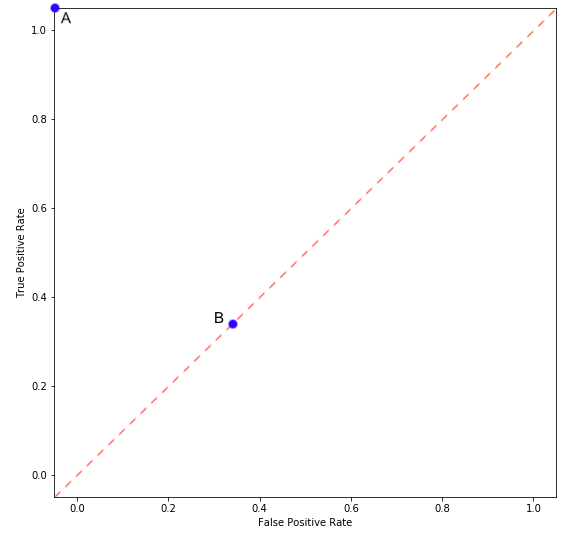
\includegraphics[scale=0.45]{Tesi/images/ROC.png}
    \caption{ROC Example}
    \label{fig:figure_5.1}
\end{figure}

\newpage
Point $\textup{A=(0,1)}$ represents the ideal case, in which all the samples are assigned to the correct class. Point $\textup{B}$, instead, lies on the so called \textit{line of no discrimination}, whose performance is the same of a random guessing. Note that the line of no discrimination splits the ROC space into two parts: points above the line represents good classification results, while points below represents bad results (worse than random).
A way to asses the overall performance of a predictor is that of drawing a curve on the ROC plane by plotting its score for every possible threshold value used to discriminate between positive and negative class. Then we can finally calculate the area under the curve, obtaining the \ac{AUROC} value (also called AUC). For what it concern the medical field,according to \cite{auroc}, an AUC of 0.5 suggests no discrimination, 0.7 to 0.8 is considered acceptable, 0.8 to 0.9 is considered excellent, and more than 0.9 is considered outstanding.

\vspace{5mm}
\section{Experimental Design}
\label{sec:experimental_design}
The first experiment we conducted involved a single CNN, more specifically a DenseNet121. Using U-Ones as policy for dealing with uncertain labels, we trained it for 5 epochs using a training set composed by 189116 samples. The learning rate was initially set to 1e-4 and then reduced by a factor of 10 after each epoch. As objective function we used the binary cross-entropy. Then we have repeated the experiment but using U-Ones+LSR as policy for dealing with uncertain labels.
\noindent Next step was that of exploiting the diseases taxonomy, using Conditional Training. During the first phase we used a training set composed by 90954 samples and we trained the DenseNet121 network end to end, using the same set up of the previous experiments. Then we froze all the layers except the last fully connected one and we retrain the network using all the 189116 samples for 5 epochs. The same procedure has been repeated for each architecture indicated in Table \ref{table:table_4.1}, obtaining the 7 different models that we then combined exploiting different ensemble techniques.
Moreover, the networks have been used to generate the embeddings, extracted from the Global Average Pooling layer and then used to train both Random Forest and XGBoost. The hyperparameters have been tuned using a validation set composed by 1911 samples. 


\section{Experiment Results}
\label{sec:experiment_result}

We will now present and discuss the results we obtained in our experiments, using the models we have introduces in the previous chapter. We will compare each other, showing, for each one, the benefits and the downsides.

\vspace{5mm}

\subsection{Single CNN}
Our first objective was to check the effectiveness of Label Smooth Regularization and Conditional Training. Starting from a simple model, that we used as baseline, we then implemented the two strategies, checking whether they were able to bring some improvements or not.
As baseline we used a DenseNet121 architecture (the same used in \cite{irvin2019chexpert} \cite{pham2019interpreting}), trained with U-Ones policy for dealing with uncertain labels. As we can see in Figure \ref{fig:figure_5.2}, this approach was able to achieve a mean AUROC across the five diseases of 0.865 which, according to \cite{auroc}, is already a good result. The network, however, showed difficulties in recognizing the cases of Atelectasis and Cardiomegaly, while, instead, was able to identify pretty well the \acp{CXR} containing Edema and Pleural Effusion that, is worth noting, are the most balanced diseases among those we are considering (Table \ref{table:table_2}).

\begin{figure}[htbp!]
    \centering
    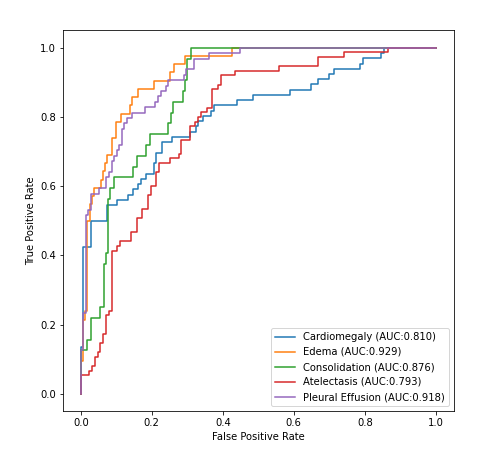
\includegraphics[scale=0.57]{Tesi/images/Results/densenet121_baseline.png}
    \caption[ROC curve for U-Ones policy]{ROC curve of DenseNet121 architecture trained with U-Ones policy}
    \label{fig:figure_5.2}
\end{figure}

\newpage

Using the Label Smooth Regularization, together with the U-Ones policy, led to an improvement in recognizing all the pathologies except for Consolidation, where the previous approach outperformed the current one (Figure \ref{fig:figure_5.3}).

\begin{figure}[htbp!]
    \centering
    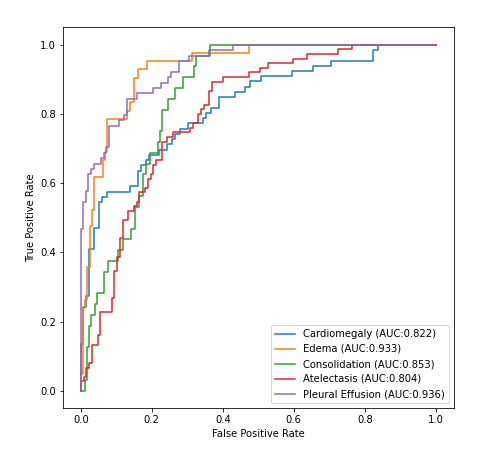
\includegraphics[scale=0.55]{Tesi/images/Results/densenet121_LSR (1).png}
    \caption[ROC curve for U-Ones+LSR policy]{ROC curve of DenseNet121 trained with U-Ones policy + Label Smooth Regularization.}
    \label{fig:figure_5.3}
\end{figure}


The use of Conditional Training, instead, gave a big improvement in identifying the cases of Atelectasis and Consolidation (Figure \ref{fig:figure_5.4}), with the downside of slightly worsening the performance over the other diseases. The mean \ac{AUROC}, however, is the best obtained so far (0.876), confirming the hypothesis that using additional side information, such as dependencies among the pathologies, can help improving the overall performance of the network.
\newpage
\begin{figure}[htbp!]
    \centering
    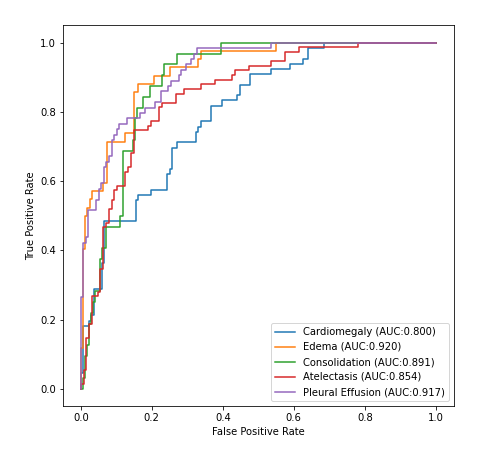
\includegraphics[scale=0.55]{Tesi/images/Results/densenet121_LSR_CT.png}
    \caption[ROC curve for U-Ones+LSR+CT policy]{ROC Curve of DenseNet121 trained with U-Ones policy + Label Smooth Regularization + Conditional Training.}
    \label{fig:figure_5.4}
\end{figure}

\vspace{5mm}

Table \ref{table:table_5.1} shows the comparison of the three different approaches we've investigated using a single CNN.

\begin{table}[h!]
\centering
\resizebox{\columnwidth}{!}{
\renewcommand{\arraystretch}{1.5}
\begin{tabular}{|l|l|l|l|l|l|l|} 
\hline
\textbf{Method} & \textbf{Atelectasis} & \textbf{Cardiomegaly} & \textbf{Consolidation} & \textbf{Edema} & \textbf{P.}~\textbf{Effusion} & \textbf{Mean}  \\
\hline
U-Ones& 0.793 & 0.810  & 0.876 & 0.929 & 0.918 & 0.865\\\hline

U-Ones+LSR & 0.804 & \textbf{0.822}  & 0.853 & \textbf{0.933} & \textbf{0.936} & 0.869\\\hline

U-Ones+LSR+CT & \textbf{0.854} & 0.800  & \textbf{0.891} & 0.920 & 0.917 & \textbf{0.876}\\ 
\hline
\end{tabular}
}
\caption[AUROC comparison for different training policies on DenseNet121]{AUROC values obtained using DenseNet121 as architecture and the approaches indicated in the \textbf{Method} column. For each label, the highest AUROC is boldfaced.}
\label{table:table_5.1}
\end{table}



\subsection{CNN Ensemble}

 Table \ref{table:table_5.2} shows the results achieved by the other \ac{CNN} architectures trained using U-Ones+LSR+CT policy. The mean \acp{AUROC} are very similar among each other and they all present analogous behaviour in distinguishing the individual diseases: the greatest difficulties are encountered while recognizing the cases of Cardiomegaly, while they all achieve the best results identifying Edema and Pleural Effusion. The results we obtained confirm the fact that there is no an architecture outperforming all the others on each pathology. Consider, for example, the VGG19 network: it achieved the best result in recognizing Consolidation and Pleural Effusion but, instead, its performance on Cardiomegaly is the worst. 

\begin{table}[h!]
\centering
\resizebox{\columnwidth}{!}{
\renewcommand{\arraystretch}{1.5}
\begin{tabular}{|l|l|l|l|l|l|l|} 
\hline
\textbf{Model} & \textbf{Atelectasis} & \textbf{Cardiomegaly} & \textbf{Consolidation} & \textbf{Edema} & \textbf{P.}~\textbf{Effusion} & \textbf{Mean}  \\
\hline
DenseNet121& \textbf{0.854} & \textbf{0.800}  & 0.891 & 0.920 & 0.917 & \textbf{0.876}\\ \hline

DenseNet169& 0.850 & 0.795  & 0.882 & \textbf{0.936} & 0.915 & \textbf{0.876}\\ \hline

DenseNet201& 0.834 & 0.791  & 0.881 & 0.917 & 0.925 & 0.870\\ \hline

InceptionResNetV2& 0.816 & 0.784  & 0.897 & 0.925 & 0.919 & 0.869\\ \hline

Xception& 0.841 & 0.770  & 0.880 & 0.909 & 0.924 & 0.865\\ \hline

VGG16& 0.843 & 0.772  & 0.898 & 0.932 & 0.919 & 0.873\\ \hline

VGG19& 0.843 & 0.769  & \textbf{0.900} & 0.927 & \textbf{0.933} & 0.874\\ \hline

\end{tabular}
}
\caption[\acp{CNN} AUROC results]{AUROC values obtained with the \acp{CNN} indicated in the \textbf{Model} column.}
\label{table:table_5.2}
\end{table}

Once we trained the different networks, we tried to improve the overal diagnostic capability by combining them. Figures \ref{fig:figure_5.5} and \ref{fig:figure_5.6} show, respectively, the results of applying simple Average and Entropy Weighted Average as aggregation methods.  As we can see, both the approaches helped improving the model's ability to recognize each of the five pathologies. More specifically, as we can see from Table \ref{table:table_5.3}, making an entropy weighted average that took care of each model's accuracy turned out to be a successful aggregation strategy, leading to a mean \ac{AUROC} of 0.889, a result that slightly outperformed the simple average approach. 



\begin{figure}[htbp!]
    \centering
    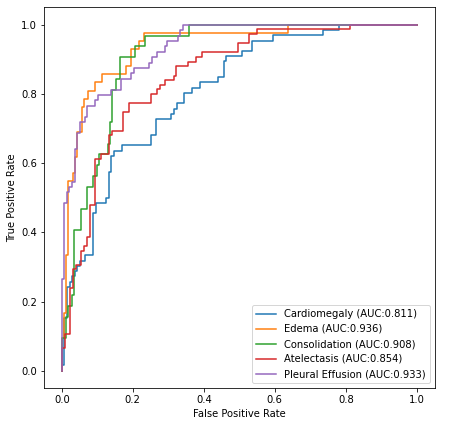
\includegraphics[scale=0.55]{Tesi/images/Results/nn_average.png}
    \caption[ROC curve for CNN average ensemble]{ROC curve of the \acp{CNN} ensemble  computed using simple average.}
    \label{fig:figure_5.5}
\end{figure}

\begin{figure}[htbp!]
    \centering
    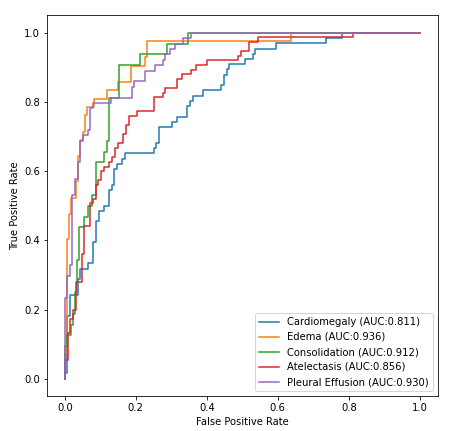
\includegraphics[scale=0.55]{Tesi/images/Results/nn_average_entropy.png}
    \caption[ROC curve for CNN weighted average ensemble]{ROC curve of the \acp{CNN} ensemble model computed using average weighted by predictions' entropy.}
    \label{fig:figure_5.6}
\end{figure}

\newpage

An aggregation approach based on Stacking, however, didn't boost the overall performance, leading to a significant improvement only in Pleural Effusion recognition.

\begin{figure}[htbp!]
    \centering
    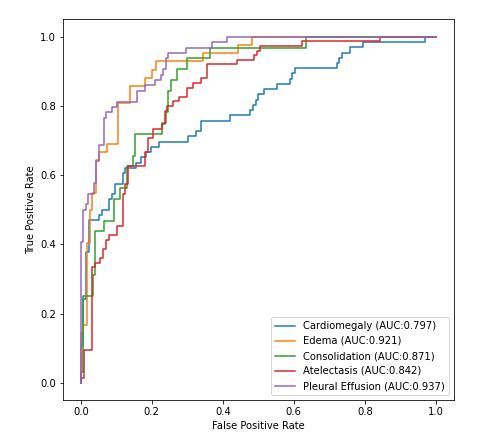
\includegraphics[scale=0.55]{Tesi/images/Results/nn_stacking.png}
    \caption[ROC curve for CNN stacking ensemble]{ROC curve of the \acp{CNN} ensemble model computed using stacking.}
    \label{fig:figure_5.7}
\end{figure}

Table \ref{table:table_5.3} reports the \acs{AUROC} obtained by the three ensemble policies, compared to the best results achieved using a single \ac{CNN}. We can clearly see that aggregating the predictions led to a significant improvement. In particular, making an entropy weighted average that took care of each model's accuracy turned out to be a successful aggregation strategy, leading to a mean \ac{AUROC} of 0.889, a result that slightly outperformed the simple average approach. 


\begin{table}[h!]
\centering
\resizebox{\columnwidth}{!}{
\renewcommand{\arraystretch}{1.5}
\begin{tabular}{|l|l|l|l|l|l|l|} 
\hline
\textbf{Method} & \textbf{Atelectasis} & \textbf{Cardiomegaly} & \textbf{Consolidation} & \textbf{Edema} & \textbf{P.}~\textbf{Effusion} & \textbf{Mean}  \\
\hline
Single CNN& 0.854 &0.800  & 0.900 & \textbf{0.936} & 0.933 & 0.885\\\hline

Average Ensemble& 0.854 & \textbf{0.811}  & 0.908 & \textbf{0.936} & 0.933 & 0.888\\\hline

Entropy Weighted AVG & \textbf{0.856} & \textbf{0.811}  & \textbf{0.912} & \textbf{0.936} & 0.930 & \textbf{0.889}\\\hline

Stacking & 0.842 & 0.797  & 0.871 & 0.921 & \textbf{0.937} & 0.873\\\hline

\end{tabular}
}
\caption[\acp{CNN} ensemble AUROC comparison]{AUROC values obtained using different Ensemble policies, compared to the best results achieved by a single CNN (reported in the first row). For each label, the highest AUROC is boldfaced.}
\label{table:table_5.3}
\end{table}


\subsection{Random Forest with Embedding}
\label{sec:rf_embedding_results}


Once we trained the \acp{CNN}, we used them to extract the embeddings. The first algorithm we used exploting them is Random Forest, whose results are shown in the Table \ref{table:table_5.4}.

\begin{table}[h!]
\centering
\resizebox{\columnwidth}{!}{
\renewcommand{\arraystretch}{1.5}
\begin{tabular}{|l|l|l|l|l|l|l|} 
\hline
\textbf{Model} & \textbf{Atelectasis} & \textbf{Cardiomegaly} & \textbf{Consolidation} & \textbf{Edema} & \textbf{P.}~\textbf{Effusion} & \textbf{Mean}  \\
\hline
DenseNet121& 0.851 & \textit{0.818}  & 0.885 & 0.915 & \textbf{\textit{0.945}} & \textit{0.883}\\ \hline

DenseNet169& \textit{0.855} & \textit{0.814}  & \textit{0.893} & \textbf{0.922} & \textit{0.933} & \textbf{\textit{0.884}}\\ \hline

DenseNet201& \textit{0.863} & \textit{0.814}  & 0.878 & \textbf{\textit{0.922}} & \textit{0.936} & \textit{0.882}\\ \hline

InceptionResNetV2& \textit{0.830} & 0.779  & \textit{0.898} & 0.918 & \textit{0.933} & \textit{0.872}\\ \hline

Xception& 0.831 & \textit{0.810}  & \textit{0.907} & \textit{0.913} & \textit{0.932} & \textit{0.879}\\ \hline

VGG16& \textit{0.858} & \textbf{\textit{0.822}}  & \textbf{\textit{0.913}} & 0.886 & 0.917 & \textit{0.879}\\ \hline

VGG19& \textbf{\textit{0.873}} & \textit{0.798}  & 0.895 & 0.892 & 0.917 & \textit{0.875}\\ \hline

\end{tabular}
}
\caption[Random Forest AUROC results]{AUROC values obtained with Random Forest trained using the embedding extracted from the CNN indicated in the \textbf{Model} column. For each label, the highest AUROC is boldfaced. A score written in italics means that the RF, on that label, outperformed the result achieved by its corresponding CNN, reported in Table \ref{table:table_5.2}}
\label{table:table_5.4}
\end{table}


\noindent As we can see, each of the single models we trained achieved, on average, a better result than its corresponding one (shown in Table \ref{table:table_5.2}), confirming the fact that the embeddings are actually able to capture the relevant information needed to distinguish the different diseases. 


\noindent As in the previous case, we combined the predictions carried out by the different models, investigating the same approaches used before. Figures \ref{fig:figure_5.8} and \ref{fig:figure_5.9} show the results obtained using, respectively, Average and Entropy Weighted Average as ensemble policy. 

\begin{figure}[htbp!]
    \centering
    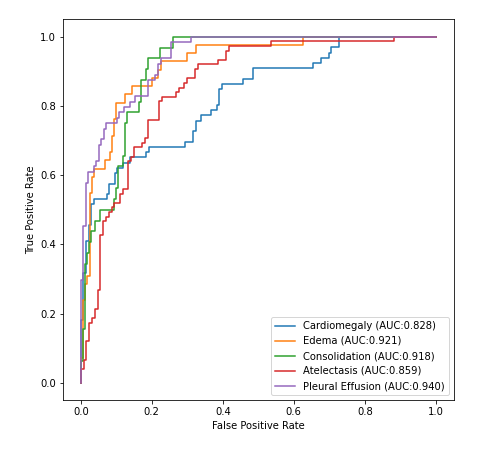
\includegraphics[scale=0.55]{Tesi/images/Results/rf_average.png}
    \caption[ROC curve for RF simple average ensemble]{ROC curve of the RF ensemble model computed using simple average.}
    \label{fig:figure_5.8}
\end{figure}

\begin{figure}[htbp!]
    \centering
    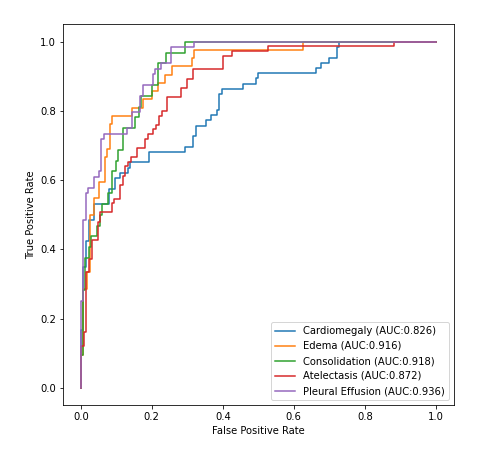
\includegraphics[scale=0.55]{Tesi/images/Results/rf_average_entropy.png}
    \caption[ROC curve for RF weighted average ensemble]{ROC curve of the RF ensemble model computed using average weighted by predictions' entropy.}
    \label{fig:figure_5.9}
\end{figure}

\noindent They both brought to a significant improvement, with the latter achieving a mean AUROC of 0.897 (Table \ref{table:table_5.5}), the highest result among those we have seen so far. 

\noindent Using stacking as aggregation method, instead, didn't help improving the diagnosis. On the contrary, this approach drastically reduced the performance on Cardiomegaly, leading to one of the worst score on that label. 

\begin{figure}[htbp!]
    \centering
    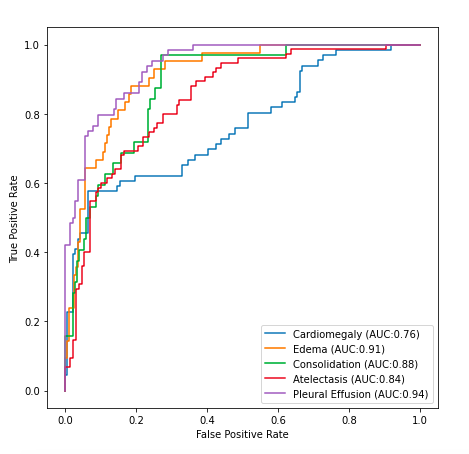
\includegraphics[scale=0.55]{Tesi/images/Results/rf_stacking.png}
    \caption[ROC curve for RF stacking ensemble]{ROC curve of the RF ensemble model computed using stacking.}
    \label{fig:figure_5.11}
\end{figure}

We can see the results of the three ensemble methods in Table \ref{table:table_5.5}, compared to the best result achieved by a single Random Forest (the one obtained by using the embedding extracted by the DenseNet169 architecture).


\begin{table}[h!]
\centering
\resizebox{\columnwidth}{!}{
\renewcommand{\arraystretch}{1.5}
\begin{tabular}{|l|l|l|l|l|l|l|} 
\hline
\textbf{Method} & \textbf{Atelectasis} & \textbf{Cardiomegaly} & \textbf{Consolidation} & \textbf{Edema} & \textbf{P.}~\textbf{Effusion} & \textbf{Mean}  \\
\hline
Single RF& 0.855 & 0.814  & 0.893 & 0.922 & 0.933 & 0.884\\\hline

Average& 0.859 & \textbf{0.828}  & \textbf{0.918} & \textbf{0.921} & \textbf{0.940} & 0.893\\\hline

Entropy Weighted AVG& \textbf{0.872} & 0.826  & \textbf{0.918} & 0.916 & 0.936 & \textbf{0.897}\\\hline

Stacking& 0.840 & 0.761  & 0.883 & 0.908 & 0.937 & 0.866\\\hline

\end{tabular}
}
\caption[\ac{RF} ensemble AUROC comparison]{AUROC values obtained using different Ensemble policies combining Random Forest models trained using the embeddings. For each label, the highest AUROC is boldfaced.}
\label{table:table_5.5}
\end{table}

Table \ref{table:table_5.6}, instead, shows the comparison between the best result achieved using Neural Networks with respect to that obtained by the embeddings. As we can clearly see, the latter is able to outperform the ensemble of \acp{CNN} in the recognition of all the diseases except for Edema.

\begin{table}[h!]
\centering
\resizebox{\columnwidth}{!}{
\renewcommand{\arraystretch}{1.5}
\begin{tabular}{|l|l|l|l|l|l|l|} 
\hline
\textbf{Method} & \textbf{Atelectasis} & \textbf{Cardiomegaly} & \textbf{Consolidation} & \textbf{Edema} & \textbf{P.}~\textbf{Effusion} & \textbf{Mean}  \\
\hline
CNNs& 0.856 & 0.811  & 0.912 & \textbf{0.936} & 0.930 & 0.889\\\hline

RF Embeddding& \textbf{0.872} & \textbf{0.826}  & \textbf{0.918} & 0.916 & \textbf{0.936} &  \textbf{0.897}\\\hline
\end{tabular}
}
\caption[CNNs and RF Embedding comparison]{AUROC values comparison between CNNs and RFs trained using embedding. For each label, the highest AUROC is boldfaced.}
\label{table:table_5.6}
\end{table}


\subsection{XGBoost}

The embeddings have been used to trained another set of models, based on XGBoost, whose results are reported in Table \ref{table:table_5.6}. All of them, except for DenseNet201, achieved results similar to those obtained with the \acp{CNN}. Random Forest, thus, seems to be more capable of exploiting the embedding to classify the \ac{CXR}.



\begin{table}[h!]
\centering
\caption[XGBoost AUROC results]{AUROC values obtained with XGBoost trained using the embedding extracted from the CNN indicated in the \textbf{Model} column.}
\resizebox{\columnwidth}{!}{
\renewcommand{\arraystretch}{1.5}
\begin{tabular}{|l|l|l|l|l|l|l|} 
\hline
\textbf{Model} & \textbf{Atelectasis} & \textbf{Cardiomegaly} & \textbf{Consolidation} & \textbf{Edema} & \textbf{P.}~\textbf{Effusion} & \textbf{Mean}  \\
\hline
DenseNet121& 0.803 & \textit{0.837}  & 0.837 & \textbf{\textit{0.944}} & \textit{0.935} & 0.871\\ \hline

DenseNet169& 0.812 & \textit{0.829}  & 0.866 & 0.916 & \textit{0.923} & 0.869\\ \hline

DenseNet201& \textbf{0.824} & \textbf{\textit{0.867}}  & 0.876 & \textit{0.920} & \textbf{\textit{0.938}} & \textbf{\textit{0.885}}\\ \hline

InceptionResNetV2& \textit{0.820} & \textit{0.792}  &\textbf{\textit{0.911}} & 0.911 & \textit{0.922} & \textit{0.871}\\ \hline

Xception& 0.803 & \textit{0.804}  & \textit{0.901} & 0.899 & 0.923 & \textit{0.866}\\ \hline

VGG16& \textit{0.800} & 0.840 & 0.849 & 0.922 & \textit{0.927} & 0.868\\ \hline

VGG19& 0.811 & \textit{0.819}  & 0.832 & 0.921 & 0.922 & 0.861\\ \hline

\end{tabular}
}
\label{table:table_5.7}
\end{table}

Combining the XGBoost models, however, the performance increased significantly with respect to using the single models alone (Figure \ref{fig:figure_5.11} and \ref{fig:figure_5.12}). In particular, differently from the previous approaches, by combining the XGBoost predictions the system is able to achieve good results also on Cardiomegaly that, according to the previous results, was one of the most difficult pathology to identify.


\begin{figure}[htbp!]
    \centering
    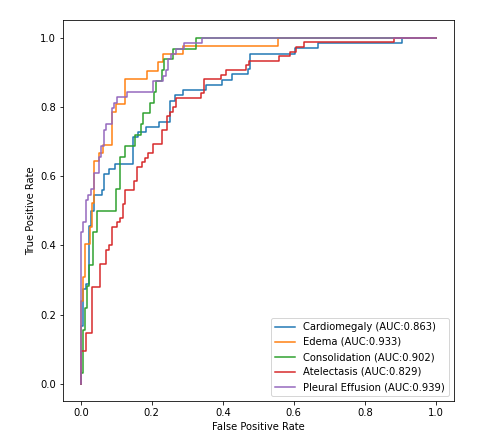
\includegraphics[scale=0.55]{Tesi/images/Results/xgb_average.png}
    \caption[ROC curve for XGBoost simple average ensemble]{ROC curve of the XGBoost ensemble model computed using simple average.}
    \label{fig:figure_5.11}
\end{figure}

\newpage

\begin{figure}[t!]
    \centering
    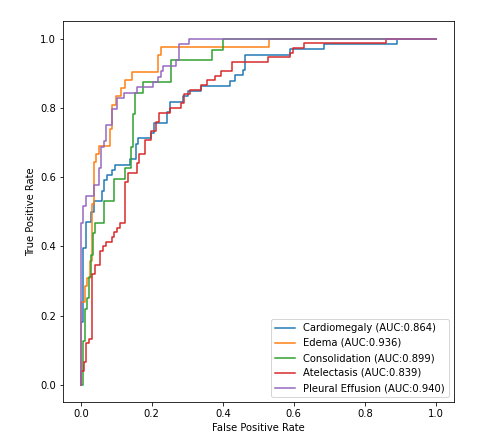
\includegraphics[scale=0.55]{Tesi/images/Results/xgb_average_entropy.png}
    \caption[ROC curve for XGBoost weighted average ensemble]{ROC curve of the XGBoost ensemble model computed using average weighted by predictions' entropy.}
    \label{fig:figure_5.12}
\end{figure}

The results obtained after the aggregation are summarized in the Table \ref{table:table_5.8}, along with the best result obtained using \acs{CNN}. Again, the use of the embedding is able to outperform the results achieved using the full images.

\begin{table}[h!]
\centering
\resizebox{\columnwidth}{!}{
\renewcommand{\arraystretch}{1.5}
\begin{tabular}{|l|l|l|l|l|l|l|} 
\hline
\textbf{Method} & \textbf{Atelectasis} & \textbf{Cardiomegaly} & \textbf{Consolidation} & \textbf{Edema} & \textbf{P.}~\textbf{Effusion} & \textbf{Mean}  \\
\hline
CNNs& \textbf{0.856} & 0.811  & \textbf{0.912} & \textbf{0.936} & 0.930 & 0.889\\\hline

XGB Average& 0.829 & 0.863  & 0.902 & 0.933 & 0.939 & 0.893\\\hline

XGB Entropy Weighted AVG& 0.839 & \textbf{0.864}  & 0.899 & \textbf{0.936} & \textbf{0.940} & \textbf{0.896}\\\hline

\end{tabular}
}
\caption[CNNs and XGBoost ensemble AUROC comparison]{AUROC values obtained using different Ensemble policies combining XGBoost models trained using the embeddings. For each label, the highest AUROC is boldfaced.}
\label{table:table_5.8}
\end{table}



\subsection{Final Results}

The final predictions have been obtained by making a simple average of the three different ensembles (CNN, RF and XGBoost), each one computed using a weighted average ensemble policy and trained using U-Ones+LSR+CT. In Figure \ref{fig:figure_5.13} are reported the ROCs curve obtained, one for each pathology.

\begin{figure}[h!]
    \centering
    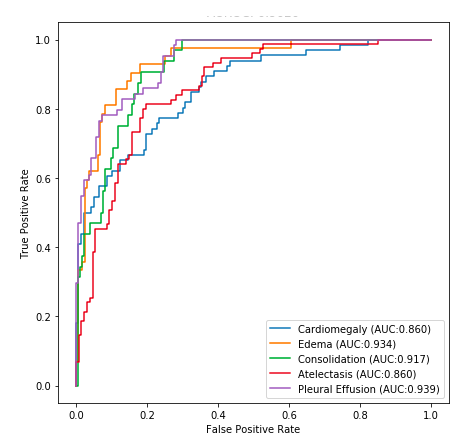
\includegraphics[scale=0.55]{Tesi/images/Results/Final Model.png}
    \caption[Final model ROC]{ROC curve of the final model, obtained by aggregating the ensembling of CNN, RF and XGBoost.}
    \label{fig:figure_5.13}
\end{figure}


Table \ref{table:table_5.9}, finally, reports a summary of all the results we obtained so far, showing the model from which we started (DenseNet121+U-Ones), the best models obtained using CNNs, RFs and XGBoost (trained using U-Ones+LSR+CT), their ensemble (obtained using Entropy Weighted Average as ensemble policy) and the final model, that achieved a mean AUROC of 0.902. The biggest improvement, with respect to the starting point, is the one involving Atelectasis and Cardiomegaly, that are the diseases on which the initial model performed worse. 

\begin{table}[h!]
\centering
\resizebox{\columnwidth}{!}{
\renewcommand{\arraystretch}{1.5}
\begin{tabular}{|l|l|l|l|l|l|l|} 
\hline
\textbf{Method} & \textbf{Atelectasis} & \textbf{Cardiomegaly} & \textbf{Consolidation} & \textbf{Edema} & \textbf{P.}~\textbf{Effusion} & \textbf{Mean}  \\
\hline
DenseNet121 + U-Ones& 0.793 & 0.810  & 0.876 & 0.929 & 0.918 & 0.865\\\hline

CNN (DenseNet121)& 0.854 & 0.800  & 0.891 & 0.920 & 0.917 & 0.876\\\hline


RF (DenseNet169)& 0.855 & 0.814  & 0.893 & 0.922 & 0.933 & 0.884\\\hline

XGB (DenseNet201)& 0.824 & \textbf{0.867}  & 0.876 & 0.920 & 0.938 & 0.885\\ \hline

CNN Ensemble& 0.855 & 0.811  & 0.912 & 0.936 & 0.930 & 0.889\\\hline

RF Ensemble& \textbf{0.872} & 0.826  & \textbf{0.918} & 0.916 & 0.936 & 0.897\\\hline

XGB Ensemble& 0.839 & 0.864  & 0.899 & \textbf{0.936} & \textbf{0.940} & 0.896\\\hline

\rowcolor[rgb]{0.851,0.851,0.851}Final Ensemble& 0.860 & 0.860  & 0.917 & 0.934 & 0.939 & \textbf{0.902}\\\hline

\end{tabular}
}
\caption[Final AUROC]{AUROC comparison of the different approaches investigated in this work. Note that, for the single models, we reported only the one achieving the highest mean result (the name of the corresponding architecture is reported between brackets).}
\label{table:table_5.9}
\end{table}

\newpage
Our final model was able to outperform, on average, the one proposed by the author of the Chexpert dataset \cite{irvin2019chexpert}, whose results are shown in the Table \ref{table:table_5.10}

\begin{table}[h!]
\centering
\resizebox{\columnwidth}{!}{
\renewcommand{\arraystretch}{1.5}
\begin{tabular}{|l|l|l|l|l|l|l|} 
\hline
\textbf{Model} & \textbf{Atelectasis} & \textbf{Cardiomegaly} & \textbf{Consolidation} & \textbf{Edema} & \textbf{P.}~\textbf{Effusion} & \textbf{Mean}  \\
\hline
Chexpert& 0.821 & 0.854  & \textbf{0.937} & 0.928 & 0.936 & 0.895\\\hline

Ours& \textbf{0.860} & \textbf{0.860}  & 0.917 & \textbf{0.934} & \textbf{0.939} & \textbf{0.902}\\\hline
\end{tabular}
}
\caption[Chexpert AUROC comparison]{AUROC comparison with Chexpert author's model (for simplicity we only report, among the results they obtained, the one with the highest mean AUROC).}
\label{table:table_5.10}
\end{table}

We weren't able, however, to outperform the system developed by Pham et al. \cite{pham2019interpreting}, whose results are reported in Table \ref{table:table_5.11}. Nevertheless we achieved good results using different approaches and, in particular, we show that using the embedding is possible to develop a \ac{CXR} diseases classifier using algorithm that are computationally much less expensive than \acp{CNN}.


\begin{table}[h!]
\centering
\resizebox{\columnwidth}{!}{
\renewcommand{\arraystretch}{1.5}
\begin{tabular}{|l|l|l|l|l|l|l|} 
\hline
\textbf{Model} & \textbf{Atelectasis} & \textbf{Cardiomegaly} & \textbf{Consolidation} & \textbf{Edema} & \textbf{P.}~\textbf{Effusion} & \textbf{Mean}  \\
\hline
Ours& 0.860 & 0.860  & 0.917 & 0.934 & 0.939 & 0.902\\\hline

Pham et al.& \textbf{0.909} & \textbf{0.910}  & \textbf{0.957} & \textbf{0.958} & \textbf{0.964} & \textbf{0.940}\\\hline

\end{tabular}
}
\caption[Pham et al. AUROC comparison ]{AUROC comparison with Pham et al. model.}
\label{table:table_5.11}
\end{table}

\subsubsection{Confusion Matrices}

Figure \ref{fig:figure_5.14} shows the confusion matrices for the five diseases, a more intuitive way to display the output of our model. For each pathology we used a different decision threshold. They have been tuned using the validation set, by taking, for each disease, the average output activation. We also defined a region of uncertainty around the threshold, in which the model abstains from taking a decision, allowing it to express its opinion only when it's sure about it. In this way we try to limit as much as possible the number of incorrect predictions that, in this field, could be very dangerous. As we can see, the best performance is that involving Pleural Effusion, where the model is able to correctly classify 170 out of 202 diseases. The worst confusion matrix, instead, is probably the one involving Cardiomegaly, where there are 31 False Negative (i.e cases in which the disease in present but the model is not able to identify it).
\vspace{7mm}

\begin{figure}[h!]
\begin{tabular}{cc}
  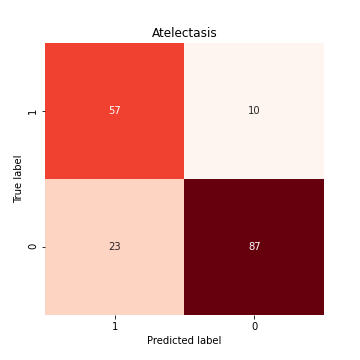
\includegraphics[width=69mm]{Tesi/images/Results/Atelectasis_cf.png} &   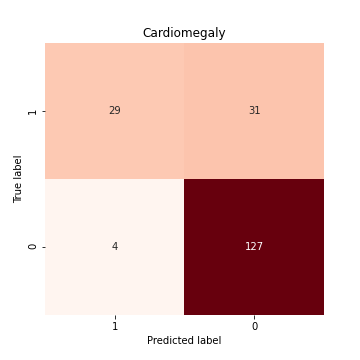
\includegraphics[width=69mm]{Tesi/images/Results/Cardiomegaly_cf.png} \\
\footnotesize{Uncertain: 25} & \footnotesize{Uncertain: 11} \\[6pt]
\multicolumn{2}{c}{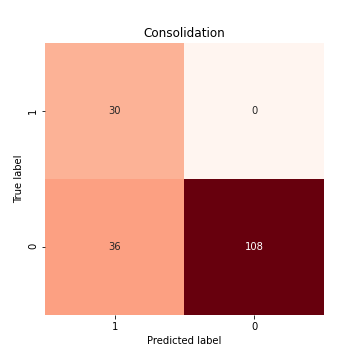
\includegraphics[width=69mm]{Tesi/images/Results/Consolidation_cf.png} }\\
\multicolumn{2}{c}{\footnotesize{Uncertain: 28}}
\end{tabular}
\end{figure}

\begin{figure}[h!]
\begin{tabular}{cc}
  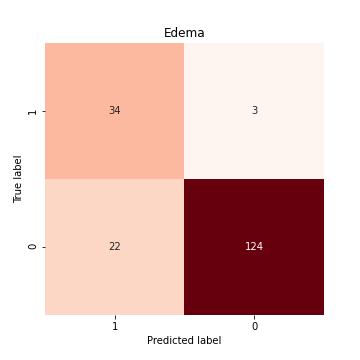
\includegraphics[width=69mm]{Tesi/images/Results/Edema_cf.png} &   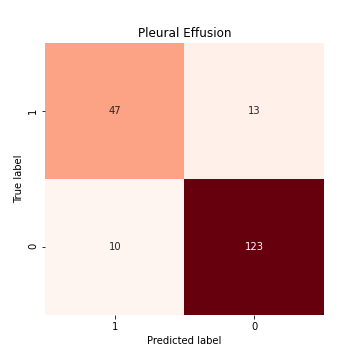
\includegraphics[width=69mm]{Tesi/images/Results/Pleural Effusion_cf.png} \\
\footnotesize{Uncertain: 19} & \footnotesize{Uncertain: 9} \\[6pt]
\end{tabular}
\caption{Confusion Matrices}
\label{fig:figure_5.14}
\end{figure}





\section{Class Activation Map}
\label{sec:cam_results}
We will now show some samples of the Class Activation Maps that have been generated. Differently from previous works, we also provided, together with the \ac{CAM}, a method to automatically extract a bounding box surrounding the area interested by the disease. Given the fact that it's hard to evaluate their goodness without having a medical background, we checked out how the model behaves in localizing the Support Devices, more easily identifiable also by a non expert eye. In Figure \ref{fig:figure_5.15} we can clearly see that the model is able to surround the medical device positioned in patient's chest.

\vspace{10mm}

\begin{figure}[htbp!]
\centering
\begin{tabular}{ccc}
 &\textbf{Support Device}& \\
\vspace{2mm}
  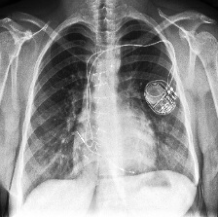
\includegraphics[width=35mm]{Tesi/images/CAMs/CAM2/image.png} &   
  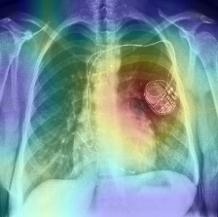
\includegraphics[width=35mm]{Tesi/images/CAMs/CAM2/image_cam.png} &   
  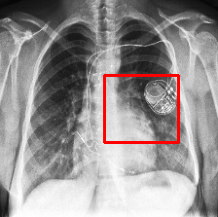
\includegraphics[width=35mm]{Tesi/images/CAMs/CAM2/image_bbox.png} \\
\footnotesize{CXR} & \footnotesize{CAM} & \footnotesize{Bounding Box} \\[6pt]
\end{tabular}
\caption[Support Device CAM-1]{}
\label{fig:figure_5.15}
\end{figure}


\begin{figure}[htbp!]
\centering
\begin{tabular}{ccc}
 &\textbf{Support Device}& \\
\vspace{2mm}
  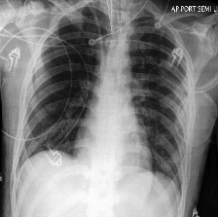
\includegraphics[width=35mm]{Tesi/images/CAMs/CAM1/image.png} &   
  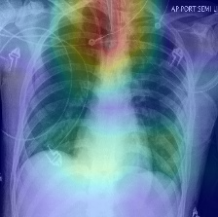
\includegraphics[width=35mm]{Tesi/images/CAMs/CAM1/image_cam.png} &   
  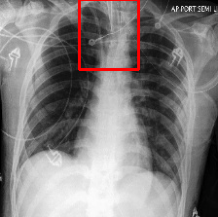
\includegraphics[width=35mm]{Tesi/images/CAMs/CAM1/image_bbox.png} \\
\footnotesize{CXR} & \footnotesize{CAM} & \footnotesize{Bounding Box} \\[6pt]
\end{tabular}
\caption[Support Device CAM-2]{}
\label{fig:figure_5.16}
\end{figure}

\begin{figure}[htbp!]
\centering
\begin{tabular}{ccc}
 &\textbf{Support Device}& \\
\vspace{2mm}
  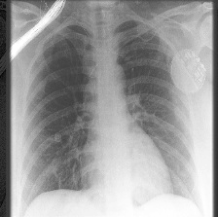
\includegraphics[width=35mm]{Tesi/images/CAMs/CAM3/image.png} &   
  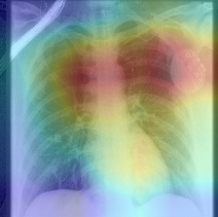
\includegraphics[width=35mm]{Tesi/images/CAMs/CAM3/image_cam.png} &   
  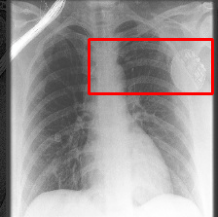
\includegraphics[width=35mm]{Tesi/images/CAMs/CAM3/image_bbox.png} \\
\footnotesize{CXR} & \footnotesize{CAM} & \footnotesize{Bounding Box} \\[6pt]
\end{tabular}
\caption[Support Device CAM-3]{}
\label{fig:figure_5.17}
\end{figure}


\begin{figure}[htbp!]
\centering
\begin{tabular}{ccc}
 &\textbf{Atelectasis}& \\
\vspace{2mm}
  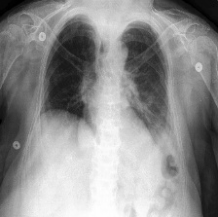
\includegraphics[width=35mm]{Tesi/images/CAMs/CAM4/image.png} &   
  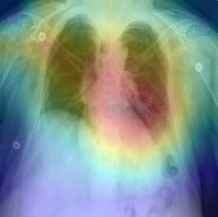
\includegraphics[width=35mm]{Tesi/images/CAMs/CAM4/image_cam.png} &   
  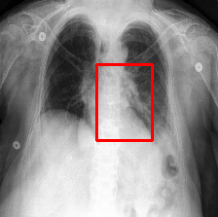
\includegraphics[width=35mm]{Tesi/images/CAMs/CAM4/image_bbox.png} \\
\footnotesize{CXR} & \footnotesize{CAM} & \footnotesize{Bounding Box} \\[6pt]
\end{tabular}
\caption[Atelectasis CAM-1]{}
\label{fig:figure_5.18}
\end{figure}

\begin{figure}[htbp!]
\centering
\begin{tabular}{ccc}
 &\textbf{Atelectasis}& \\
\vspace{2mm}
  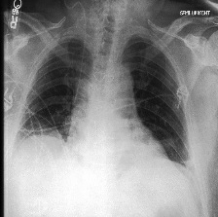
\includegraphics[width=35mm]{Tesi/images/CAMs/CAM5/image.png} &   
  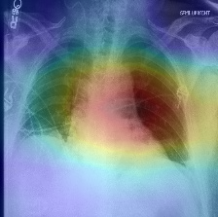
\includegraphics[width=35mm]{Tesi/images/CAMs/CAM5/image_cam.png} &   
  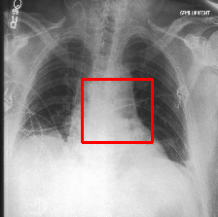
\includegraphics[width=35mm]{Tesi/images/CAMs/CAM5/image_bbox.png} \\
\footnotesize{CXR} & \footnotesize{CAM} & \footnotesize{Bounding Box} \\[6pt]
\end{tabular}
\caption[Atelectasis CAM-2]{}
\label{fig:figure_5.19}
\end{figure}


\begin{figure}[htbp!]
\centering
\begin{tabular}{ccc}
 &\textbf{Cardiomegaly}& \\
\vspace{2mm}
  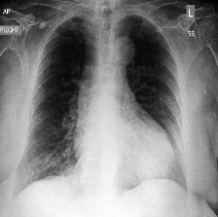
\includegraphics[width=35mm]{Tesi/images/CAMs/CAM6/image.png} &   
  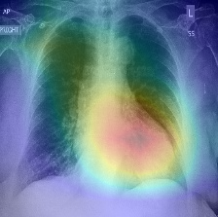
\includegraphics[width=35mm]{Tesi/images/CAMs/CAM6/image_cam.png} &   
  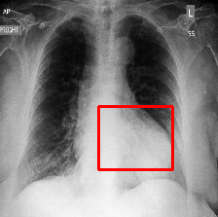
\includegraphics[width=35mm]{Tesi/images/CAMs/CAM6/image_bbox.png} \\
\footnotesize{CXR} & \footnotesize{CAM} & \footnotesize{Bounding Box} \\[6pt]
\end{tabular}
\caption[Cadiomegaly CAM-1]{}
\label{fig:figure_5.20}
\end{figure}

\begin{figure}[htbp!]
\centering
\begin{tabular}{ccc}
 &\textbf{Cardiomegaly}& \\
\vspace{2mm}
  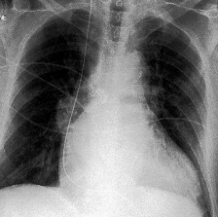
\includegraphics[width=35mm]{Tesi/images/CAMs/CAM7/image.png} &   
  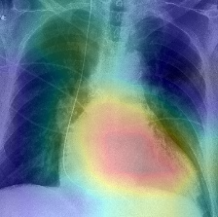
\includegraphics[width=35mm]{Tesi/images/CAMs/CAM7/image_cam.png} &   
  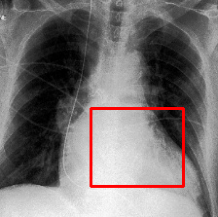
\includegraphics[width=35mm]{Tesi/images/CAMs/CAM7/image_bbox.png} \\
\footnotesize{CXR} & \footnotesize{CAM} & \footnotesize{Bounding Box} \\[6pt]
\end{tabular}
\caption[Cadiomegaly CAM-2]{}
\label{fig:figure_5.21}
\end{figure}


\begin{figure}[htbp!]
\centering
\begin{tabular}{ccc}
 &\textbf{Consolidation}& \\
\vspace{2mm}
  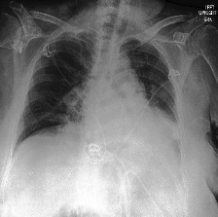
\includegraphics[width=35mm]{Tesi/images/CAMs/CAM8/image.png} &   
  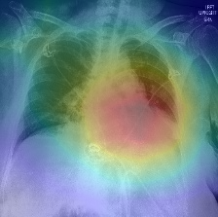
\includegraphics[width=35mm]{Tesi/images/CAMs/CAM8/image_cam.png} &   
  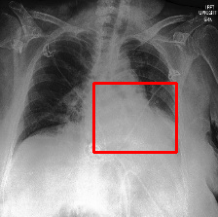
\includegraphics[width=35mm]{Tesi/images/CAMs/CAM8/image_bbox.png} \\
\footnotesize{CXR} & \footnotesize{CAM} & \footnotesize{Bounding Box} \\[6pt]
\end{tabular}
\caption[Consolidation CAM-1]{}
\label{fig:figure_5.22}
\end{figure}

\newpage

\begin{figure}[htbp!]
\centering
\begin{tabular}{ccc}
 &\textbf{Consolidation}& \\
\vspace{2mm}
  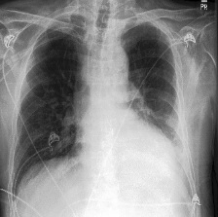
\includegraphics[width=35mm]{Tesi/images/CAMs/CAM9/image.png} &   
  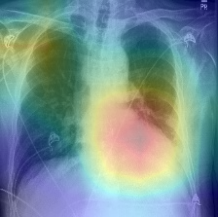
\includegraphics[width=35mm]{Tesi/images/CAMs/CAM9/image_cam.png} &   
  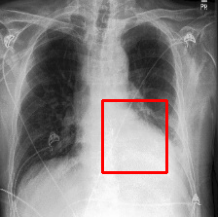
\includegraphics[width=35mm]{Tesi/images/CAMs/CAM9/image_bbox.png} \\
\footnotesize{CXR} & \footnotesize{CAM} & \footnotesize{Bounding Box} \\[6pt]
\end{tabular}
\caption[Consolidation CAM-2]{}
\label{fig:figure_5.23}
\end{figure}

\begin{figure}[htbp!]
\centering
\begin{tabular}{ccc}
 &\textbf{Edema}& \\
\vspace{2mm}
  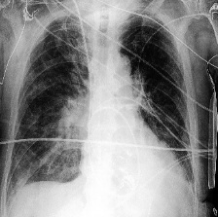
\includegraphics[width=35mm]{Tesi/images/CAMs/CAM10/image.png} &   
  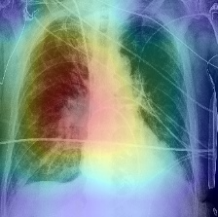
\includegraphics[width=35mm]{Tesi/images/CAMs/CAM10/image_cam.png} &   
  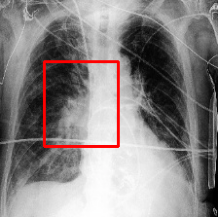
\includegraphics[width=35mm]{Tesi/images/CAMs/CAM10/image_bbox.png} \\
\footnotesize{CXR} & \footnotesize{CAM} & \footnotesize{Bounding Box} \\[6pt]
\end{tabular}
\caption[Edema CAM-1]{}
\label{fig:figure_5.24}
\end{figure}



\begin{figure}[htbp!]
\centering
\begin{tabular}{ccc}
 &\textbf{Edema}& \\
\vspace{2mm}
  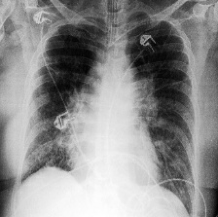
\includegraphics[width=35mm]{Tesi/images/CAMs/CAM11/image.png} &   
  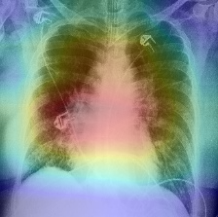
\includegraphics[width=35mm]{Tesi/images/CAMs/CAM11/image_cam.png} &   
  \includegraphics[width=35mm]{Tesi/images/CAMs/CAM11/image_bbox.png} \\
\footnotesize{CXR} & \footnotesize{CAM} & \footnotesize{Bounding Box} \\[6pt]
\end{tabular}
\caption[Edema CAM-2]{}
\label{fig:figure_5.25}
\end{figure}

\newpage

\begin{figure}[htbp!]
\centering
\begin{tabular}{ccc}
 &\textbf{Pleural Effusion}& \\
\vspace{2mm}
  \includegraphics[width=35mm]{Tesi/images/CAMs/CAM12/image.png} &   
  \includegraphics[width=35mm]{Tesi/images/CAMs/CAM12/image_cam.png} &   
  \includegraphics[width=35mm]{Tesi/images/CAMs/CAM12/image_bbox.png} \\
\footnotesize{CXR} & \footnotesize{CAM} & \footnotesize{Bounding Box} \\[6pt]
\end{tabular}
\caption[Pleural Effusion CAM-1]{}
\label{fig:figure_5.26}
\end{figure}

\begin{figure}[htbp!]
\centering
\begin{tabular}{ccc}
 &\textbf{Pleural Effusion}& \\
\vspace{2mm}
  \includegraphics[width=35mm]{Tesi/images/CAMs/CAM13/image.png} &   
  \includegraphics[width=35mm]{Tesi/images/CAMs/CAM13/image_cam.png} &   
  \includegraphics[width=35mm]{Tesi/images/CAMs/CAM13/image_bbox.png} \\
\footnotesize{CXR} & \footnotesize{CAM} & \footnotesize{Bounding Box} \\[6pt]
\end{tabular}
\caption[Pleural Effusion CAM-2]{}
\label{fig:figure_5.27}
\end{figure}



\section{Summary}
\label{sec:chapter_5_summary}
At the beginning of this chapter we have presented the evaluation criteria we have used to assess the performance of our models. Then we have presented all the results we achieved using the approaches defined in the previous chapters, discussing them and comparing each other. Using the confusion matrices we tried to give the lecturer a more comprehensible summary about our model performances. We then compared our results with that obtained by the state of the art. Finally, we have provided some samples of the \acp{CAM} and Bounding Boxes that have been generated. In the next chapter we will give some considerations about our overall work and we will discuss some possible future works related to it.